R.F.I.D. consists of four distinct functional blocks. All functional blocks, along with the system input and outputs, are shown in relation to each other in Figure~\ref{fig:functional_diagram}. This section discusses the function of each block in relation to each other. and any significant technical specifications with which that block is associated.

% TODO: Make this Figure more readable. I know EPayne and Sheaff want larger text
% TODO: No light text (The green)
\begin{figure}[H]
    \centering
    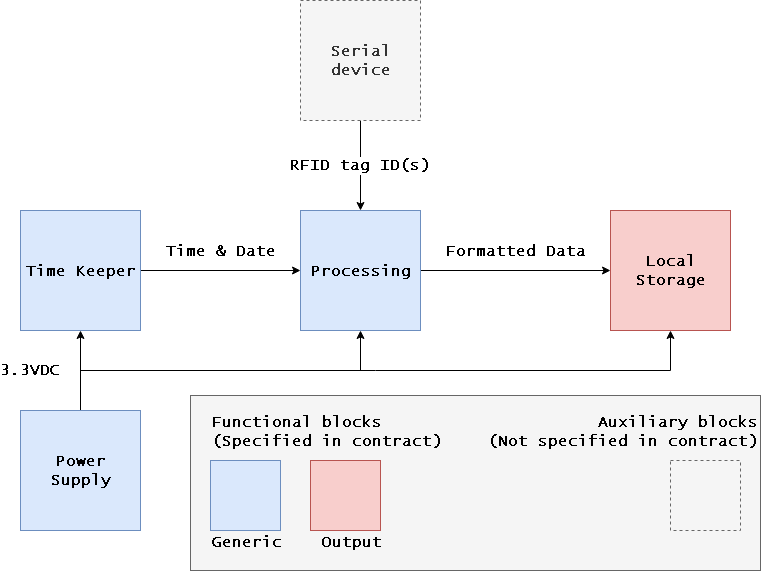
\includegraphics[width=1\textwidth]{Figures/3_breakdown/FBD.png}
    \caption{R.F.I.D. functional block diagram.}
    \label{fig:functional_diagram}
\end{figure}



R.F.I.D. receives RFID tag IDs as its system input, and outputs tag IDs, time, and date. The Power Supply block outputs a DC voltage to provide sufficient power to the Processing and Local Storage blocks. The Time Keeper block outputs time and date to the Processing block. The Processing block receives RFID tag data from an external device, and outputs tag IDs, time, and date to the Local Storage block. The final system output received by the Local Storage block is stored on a FAT formatted SD card. See Appendix B for the complete schematic.

% Dan: I editted the above paragraph
% =====================================================================================

\subsection{Power Supply}

The Power Supply block consists of a battery and a DC-DC converter. The battery provides readily accessible power for the project, while the DC-DC converter regulates the battery voltage level to provide 3.3VDC $\pm$ 10\% to provide a safe voltage level to power the Processing and Local Storage blocks. That is to say, the DC-DC converter has the onboard battery as its source and the physical contents of Processing and Local Storage blocks as its load.

\subsection{Time Keeper}
The Time Keeper block consists of a quartz crystal resonator circuit and the real-time clock portion of the microcontroller used in the project. This block is required to provide the time and date information that is stipulated in the project contract. The resonator circuit provides a 32.768kHz clock frequency to the real-time clock of the microcontroller, which lowers the provided frequency to 1Hz and keeps track of both the time and date on a second by second basis. The final time and date data are passed to the Processing block, where they are used to keep track of when RFID Tag Data is received by R.F.I.D..
% Dan: I want to check on the wording of this above parag.
% =====================================================================================


\subsection{Processing}
 The Processing block receives RFID tag data via serial communication. This block receives 3.3VDC $\pm$ 10\% from the Power Supply block. The block also outputs RFID tag data, with date and time stamps, to the Local Storage block. The Processing block consists of a microcontroller. It obtains and formats all data. It also initializes all associated peripherals and general software operation of the device. This block communicates with two devices: the external device that provides the system input and the SD card where it stores data. Lastly, this block provides the memory and computational power required to write data to the Local Storage block in accordance with a FAT format.
 
 % TODO: check if above is a good description
 
 %Among chief concerns are the fact that several communication standards are in use by the device, requiring careful clock configuration and main program organization; and the fact that the code base must be fairly compact with room for modifications as necessary for different RFID devices or outputs.


%The Processing block consists of a microcontroller that serves two purposes. It maintains communication with an external device that provides RFID tag data, and also communicates with an SD card to record data. The microcontroller also provides the memory and computation power required to write data to the Local Storage block in keeping with a FAT format.


\subsection{Local Storage}
The Local Storage block receives RFID tag IDs, date and time stamps, from the Processing block. It is powered by the Power Supply block. Data received from the Processing block is stored on a FAT file formatted SD card. This block consists of both hardware and software; it includes a software library that controls the exchange of data to and from the SD card. However, software functions account for most of this block's complexity. The primary concern is whether the data to be read or written is formatted correctly; that is, in consistent chunks and sectors with an intact BIOS Parameter Block (BPB), which is used to glean most information about a new filesystem.

%% Dan: I'm kind of confused how to approach this subsection

% 